%!TEX root =  main.tex
%!TEX encoding = UTF-8 Unicode
\chapter{嗜好の予測:まとめ}
\label{sec:hybrid}

%@@@ ハイブリッドの中の完全結合はトピックモデルや行列分解に移動
%@@@ ハイブリッドだけで単独の章にする

ここでは,協調フィルタリングと内容ベースの二つの予測手法を組み合わせたハイブリッド法について述べたあと,アルゴリズムの選択の指針について述べる.

\section{ハイブリッド法}
\label{sec:combmethod}
\index{ハイブリッド推薦システム}\index{hybrid recommender system}

\ref{sec:cfcbf}では,協調と内容ベースの2種類の推薦手法を紹介し,それぞれの長所と短所を述べた.
簡単にまとめると,協調フィルタリングは他の利用者の意見に基づいて推薦する方法で,アイテム特徴のデータベースが不要であることや,多様性の高い推薦ができるなどの利点がある.
一方,内容ベースフィルタリングは,アイテムや利用者の特徴に基づいて推薦する方法で,新規のアイテムでも推薦できるなどの利点がある.
ここで,他の利用者の意見とアイテムの特徴は相反する情報ではなく,同時に獲得できる.
そこで,互いの長所を生かすように,二つの手法を組み合わせたハイブリッド法について述べる.
このハイブリッド法の分類を,文献\cite{ej:048}の分類に,最近の研究含めて再編した分類を示す.
なお,結合が疎なものから,より密接なものへ順に並べた.
研究の動向も,より密接な結合方法へ展開しているといえるだろう.

\subsection{混合 (mixed)}

これは,協調と内容ベースの両方の手法による推薦結果を同時に混合させて提示する方法である.
どちらを採用するかは利用者に任されている.

論文の適切な査読者を探すシステム\cite{jair:01:01}は,内容ベースと協調フィルタリングの二通りの推薦機能を備える.どちらを使うかは,利用者が決める.

%PTV システム:テレビ番組の推薦.番組紹介テキストに基づく内容ベースと,他の利用者の評価を協調とのハイブリッド.新アイテムに対するcold-start問題は内容ベースでは回避できるが,利用者の評価付けが不足しているので新規利用者は内容ベースと協調のどちらも対処できない.
%協調推薦は,ニッチな番組を推薦出来る.
%PTVはスケジュールを埋める特殊な推薦なので,推薦結果の混合が可能.
%時間帯が重なったら,調停が必要だが,PTVでは内容ベース優先.
% B.Smyth and P.Cotter ``A personalized TV Listensings Service for the Digital TV Age''Knowledge-Based systems, vol.13, pp.53-59 (2000)

% ProfBuilderやPickAFlick:単純に結果を並列に示す.
% ProfBuilder
% A.M.Wasfi ``Collecting User Access Patterns for Building User Profiles and collaborative Filtering'' IUI 1999
% PickAFlick
% R.Burke, K.Hammond B.Young ``The FindMe Approach to Assisted Browsing'' IEEE Expert, vol.12, no.4, pp.32-40 (1997)

\subsection{切り替え (switching)}

何らかの規準に基づいて,内容ベースと協調の推薦手法を切り替える方法である.
嗜好データが少ないときは,比較的,疎なデータに強い協調フィルタリングを利用し,十分なデータが蓄積されれば内容ベースに切り替えるという規準がある.
また,新規アイテムに対しては,協調フィルタリングは利用できないので,内容ベースで推薦を行うが,そのアイテムへの嗜好データが蓄積されれば協調フィルタリングを使うという規準も考えられる.

%DailyLearnerは,最初は内容ベースを利用し,信頼性のある推薦ができなければ,協調推薦に切り替える.
%最近隣法による内容ベース手法を用いているためramp-up問題を回避でき,ジャンルにわたる推薦も可能になる.
% Adaptive Personalization for the Mobile Web -- Michael J. Pazzani WWW2000 Workshop: Devday: Mobile Web Track

% Tran\&Cohenの方法では,過去の評価と各推薦手法との一致によって切り替える.
% T.Tran & R.Cohen "Hybrid Recommender Systems for Electronic Commerce" AAAI workshop, 2000

\subsection{メタ推薦 (meta-recommendation)}

メタ推薦とは個別に得られた各推薦手法の推薦結果を統合する方法である.
情報検索で,複数の検索結果を統合するメタ検索エンジン\cite{www:01:01}と同様の手法である.
この方法には,各手法を改造する必要がないため実装が容易である利点がある.
%評価値を予測し易いアイテムとそうでないものとが,各手法ごとに一般には異なるが,全てのアイテムが同様に扱われる問題がある.

P-Tango\cite{misc:092}では,内容ベースと協調のスコアの重み付線形和を,全体のスコアとする.
内容ベースと協調のスコアの重みは初期的には同じである.
その後,推薦結果を利用者が受け入れたかどうかのフィードバックに基づいて,それぞれの手法の重みを変化させている.

Pazzaniの方法\cite{ej:050}では,各手法による推薦リストの1〜5位に,それぞれ5〜1点を与え,各アイテムの総点数に基づいて最終的な推薦順位を決定するBorda count法\cite{eb:042:05}によって統合する.

TiVo\cite{kdd:04:11}では,基本的には予測評価値で整列してアイテムを提示するが,評価値が同じなら協調フィルタリングの方を内容ベースより上位に表示する.

\subsection{縦続 (cascade)}

この手法では,最初の段階で候補集合を生成し,次段階でその候補集合から詳細な推薦をする.候補を限定することで,推薦を高速化し,また,条件から大きくかけ離れたアイテムを推薦することを回避できる.

EntreeC\cite{ej:048}はレストランの推薦システムである.
最初の段階では,価格帯や和洋中など,希望するレストランの特徴を示した検索質問を用いて,内容ベースの手法で候補となるレストランを選び出す.
その後,協調フィルタリングによって,候補の順位付けをする.

Google News\cite{www:07:01}では,利用者が指定した言語やジャンルや,記事の新しさなどので候補記事を絞り込んだのち,協調フィルタリングでより個人化した推薦を行う.
逆に,推薦リストを提示した後に,具体的な条件でフィルタリングする手法\cite{sigir:01:01}も論じられている.
こうした簡単な条件による推薦候補の絞り込みは,実装が容易な割に利用者の満足を高めるとされているので\cite{sigir:01:01},ぜひ導入しておくべきであろう.

\subsection{特徴拡張 (feature augmentation)}

特徴拡張とは,一方の手法が出力する評価値や分類結果を,もう一方の手法の入力とするアプローチである.
上記の縦続接続では,二つの推薦器の出力を優先度をつけるが,特徴拡張では,一方の出力がもう一方の入力となる点が異なる.

Libra\cite{sigir:99:01}は書籍の推薦システムで,Amazon.comから取得した書籍情報の特徴に基づいて内容ベースの推薦を実行する.
このとき,Amazon.com内の協調フィルタリングによって抽出された関連書籍を,書籍の特徴に含めることで協調フィルタリングの要素を加えている.
協調フィルタリングにより求めた類似アイテムを,アイテムの特徴に反映させる手法はSmartPad\cite{dmkd:01:02}にも見られる.

Goodらの方法\cite{aaai:99:01}は,人間の標本利用者の他に,アイテムの特徴に基づいて嗜好を判断する仮想エージェント利用者も参加させて協調フィルタリングをする.
仮想エージェント利用者には,特定のジャンルの映画に高い評価値を与えるものなどがある.こうして,内容ベースの推薦の要素を加える.

%\subsubsection{特徴結合}
%協調情報を各事例の特徴として,元のデータに追加して内容ベースをする方法
%Basuらの方法:利用者の評価値と内容の特徴の両方を用いる.精度は向上しないが,再現率は向上.また,両方の手法を同時に利用することで,アイテムを評価付けしている利用者数の少なさに影響されにくい.
% Basu@AAAI1998
% C.Basu H.Hirsh W.Cohen ``Recommendation as Classification: Using Social and Content-Based Information in Recommendation'' 15thAAAI (1998)

\subsection{抽象情報 (abstraction)}

これは,他の利用者の嗜好データや各種の内容データを,ベクトルや確率分布の形式の,メタレベルの抽象的な情報に変換し,別の推薦器に入力する方法である.
特徴拡張とは,推薦結果そのものを受け渡さない点が異なる.
%特徴拡張は出力をそのまま他の推薦器への入力とするが,メタレベルでは生成されたモデルや特徴を別の推薦器への入力とする.
%内容ベースで利用者の関心を表す情報を生成し,この情報の類似性に基づいて協調フィルタリングを実行する.

Fab\cite{macm:97:02}は,各利用者ごとに,内容ベースの手法で利用者プロファイル,すなわち,利用者が好むアイテムの特徴を生成する.
利用者の類似性をこの利用者プロファイルの類似性で測り,類似した利用者が好むアイテムを活動利用者に推薦する.
同様の手法は\cite{ej:050}でも利用されている.

Leeの方法\cite{icml:01:01}は,\ref{sec:clustermodel}のクラスタモデルの協調フィルタリングで,各クラスタ内のモデルを内容ベースで生成する.
%なお,一人の利用者が複数のクラスタに部分的に所属するソフトなクラスタリングにより灰色の羊問題(\ref{sec:clustermodel})を避けている.
%また,アイテムの特徴の線形モデルにオンライン学習を適用することで内容ベースの予測をしている.

文献\cite{uai:03:03}では階層ベイズに基づく手法が提案されている.活動利用者の嗜好はアイテムの特徴ベクトル$\bff$が与えられたときの評価値の事後分布$\pb{r_{ay}|\bff_y,\bfTheta}$で予測する.
すなわち,内容ベースの枠組みに基づく推薦である.
しかし,ここではパラメータ$\bfTheta$の事前分布に無情報事前分布を用いないことでハイブリッド化をする.
この事前分布には,利用者DBの嗜好に依存した分布 $\pb{\bfTheta|\bfR}$,
すなわち,他の利用者の嗜好データに基づく協調フィルタリングの要素をもつものを用いる.

%利用者とアイテム両方の特徴\cite{misc:091}を使っているので協調と内容ベースの両方を使っているとはいえないと思う -- 神嶌
%Condliffの方法:内容ベースを単純ベイズで実現し,その分類器のパラメータを回帰によって利用者間で連結する.

% LaboUr:事例ベースの内容ベース手法で利用者プロファイルを作り,これらを協調推薦の枠組みで比較.
% I.Schwab A.Kobsa I.Koychev ``Learning User Interests through Positive Examples Using ContentAnalysis and Collaborotive Filtering'' UserModeling and User Adapted Interaction

\subsection{完全結合 (total integration)}

完全結合では,結合される手法に前後関係がなく,他の利用者の情報と内容情報とを同等のレベルでモデル化する.

\ref{sec:probmodel}の共起型確率モデルでは,アイテムの特徴などを容易に導入できる柔軟性があると述べた.
こうした拡張には\cite{uai:01:01,ijcai:05:01,trieice:06:04,tripsj:06:02,tieice:07:02}などがある.
一例を挙げよう.
図\ref{fig:latentmodel}(a)の利用者$x$とアイテム$y$だけを考慮するモデルに,アイテムの特徴ベクトル$\bff=\paren{f_1,\ldots,f_p}$を
導入する場合を述べる.
これは式\eqref{eq:plsamodel}に新たな項$\pb{\bff|z}$を追加して行う.
そして,次の同時確率に対する尤度を最大化することでパラメータは学習できる.
\[
 \pb{x,y,\bff} = \sum_{z\in\calZ} \pb{z|x} \pb{y|z}\pb{\bff|z}\pb{z}
\]
特徴ベクトル$\bff$の要素数が一つであれば,離散値なら多項分布で,連続値ならガウス分布などでモデル化できる.
もし要素数が二つ以上であれば,多変量ガウス分布などが利用できる.
また,$z$が与えられたときに$\bff$の各要素は独立との単純ベイズの仮定のもとで,$\pb{\bff|z}=\prod_i\pb{f_i|z}$などとモデル化してもよい.

\begin{figure}
\centering
\fbox{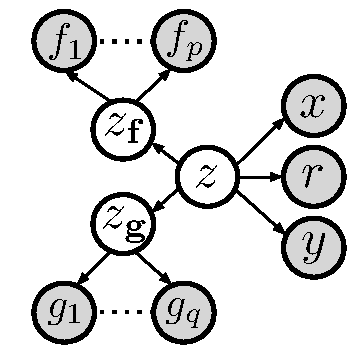
\includegraphics[width=0.6\fullwidth]{combined-topicmodel}}
\caption{ハイブリッド型のトピックモデル\cite{trieice:06:04}}
\label{fig:combined-topicmodel}
\end{figure}

文献\cite{trieice:06:04}では,アイテムの特徴$\bff$に加え,利用者の個人属性特徴や,利用意図などの特徴$\bfg=\paren{g_1,\ldots,g_q}$を加えた図\ref{fig:combined-topicmodel}のようなモデルを提案している.
これをまとめると次式のようになる.
\begin{multline*}
\pb{x,y,r,\bff,\bfg} =
 \pb{z}\pb{x|z}\pb{y|z}\pb{r|z}\\
\paren{\pb{z_\bff|z}\prod_i^p\pb{f_i|z_\bff}}
\paren{\pb{z_\bfg|z}\prod_j^q\pb{g_j|z_\bfg}}
\end{multline*}
%
このように,潜在変数を用いたトピックモデルには,推薦に関係するさまざまな要素を自在に導入できる柔軟性がある.
モデルを与えれば,EMアルゴリズムなどによりパラメータを学習できる.
いろいろなモデルの中から,集めたテストデータに,機械学習でのモデル選択の手法を適用して,最終的に利用するモデルを最終的に選べばよい.

もう一つの完全結合の手法として,関数モデルにカーネルを導入する\cite{icml:04:06}の方法を紹介する.
この方法では,順序回帰問題に帰着させてモデルを獲得する.利用者$x$がアイテム$y$を好む度合いを次の関数でモデル化する.
\[
f(x,y)=\sum_{(i,j)}w(i,j)K\paren{(x,y),(i,j)}
\]
ただし,$w(i,j)$は重みである.そして,しきい値$\theta_k$について$f(x,y)\in[\theta_{r-1},\theta_r)$を満たすなら,利用者$x$のアイテム$y$に与えた評価値は$r$と予測する.
この重み$w(x,y)$としきい値$\theta_k$は,順序回帰問題のためのパーセプトロン型の学習則であるPRankアルゴリズム\cite{nips:02:01}で獲得する.
そして,$K\paren{(x,y),(i,j)}$はカーネル\cite{jb:036:00}であり,協調と内容ベースフィルタリングを結合するときに中心的な役割を果たす.
この利用者$x$とアイテム$y$の対についてのカーネルは,適当な仮定のもと,利用者とアイテムそれぞれのカーネルの積となる.
\[
 K((x,y),(i,j))=K_X(x,i)K_Y(y,j)
\]
利用者については,$x=x'$なら$1$,でなければ$0$をとるカーネル,利用者の個人属性情報の特徴量$\bfg(x)$に基づくカーネル,利用者
$x$と$i$の間の\ref{sec:user-user}の式\eqref{eq:glsim}の相関をとるカーネルなどを個々に求め,これらのカーネルの和を$K_X(x,x')$とする.
アイテムについても同様にカーネルを定義できる.
この方法では,カーネルを自由に設計できるので,いろいろな要因を考慮した推薦が可能である.
さらに,カーネルトリックが適用できるどのような関数モデルにも適用できるので,多様な応用が可能でもある.

\section{嗜好の予測手法の選択}
\label{sec:rsselect}
%@@@ アルゴリズムの最初のまとめの章に移動

嗜好の予測手法のまとめとして,予測手法の選択指針を,私見をまじえつつ列挙しておく.

最初に,協調フィルタリングか内容ベースフィルタリングかの選択について述べる.
\ref{sec:cfcbfcomp}では,両方の手法の長所と短所について論じた.
これらのうち,内容ベースにとってはアイテム特徴のデータベースを構築し,維持できるかどうかが最大の制約である.
この構築・維持コストは,人手を要するため,一般に非常に高い.
もう一方の協調フィルタリングでは,嗜好データを収集できるかが大きな制約である.
利用者に負担をかけずにその嗜好パターンを巧妙に捉える暗黙的な収集方法か,利用者に評価付けしてもらうよい動機付けが必要になる.
これらの両方の制約を満たせるならば,それぞれの長所を生かしたハイブリッドがよいだろう.

\ref{sec:systemtarget}の運用目的別では,概要推薦であれば,非個人化推薦である人気リストや,直接指定型の内容ベースとなり,利用者評価では,システム側は基本的に場を提供するだけで,予測手法は不要である.
関連アイテム推薦では,アイテム間型メモリベースの協調フィルタリングや,アイテムの特徴を用いて関連アイテムを見つけるのが一般的である.
通知サービスや緊密な個人化では,個人情報を蓄積していることが前提なので,協調フィルタリングや間接指定型の内容ベースが利用され,予測手法の役割が重要になる.

ここで,searchとexperienceいう推薦対象アイテムの種別\cite{ej:053}についてふれておこう.
searchアイテムとは,カタログの規格からの洞察によって,どれを購入するかを選択できるもので,実用品に多い.こうしたものには,基本的には直接指定型の内容ベースを利用する.
協調フィルタリングや間接指定型の内容ベースは,順位付けなどのために補助的に利用される.
後者のexperienceアイテムは,実際に試さないと判断できないもので,嗜好品などに多い.こうしたものでは,協調フィルタリングでセレンディピティを重視した推薦が有利となる.

次に,協調フィルタリング手法の中での選択について論じる.
まず最初に,どの手法も背後にいろいろな前提がある.
例えば,\ref{sec:timeseries}の定期購読を対象とした方法は,推薦ごとに利用者が決定をする通常の推薦には適用できない.
各手法の前提に,推薦システムを適用しようとする対象が合っているかどうかは定性的に検証すべきである.
\ref{sec:memory-model}で述べたように,データの更新が頻繁ならメモリベースが有利だが,そうでなければモデルベースが高速な推薦が可能である.
%文献\cite{uai:98:01}では,明示的な多段階評価ではメモリベースが,適合/不適合の二段階評価ではモデルベースが全般的に有利である.
%明確な証拠はないが,こうした傾向は一般に見られると考えを著者も支持する.
%二段階評価は,暗黙的に獲得した嗜好データが多く,未評価と不支持の区別ができない.
%これらを区別せずに不支持として処理するため,メモリベースは不利になる.
%一方,多段階評価ではモデルベースは推定すべきパラメータ数が増えるため,二段階評価に適している.
%もちろん,十分なサンプルが準備できるならば,モデルベースでも高精度な推定が可能である.

メモリベース法には,利用者間型とアイテム間があるが,予測精度よりも他の規準でどちらかを選択すべきだろう.
アイテムの更新が頻繁である場合や,セレンディピティなどについては利用者間型が有利だろう.
一方,一時的個人化をしたい場合や,利用者の入れ替わりが頻繁な場合にはアイテム間型が有利だろう.
%新規利用者に,特定のアイテム群について評価値を入力させる方法は,アイテム間型では無意味である.
%改良手法の中で,評価値平均を0にする正規化と,デフォルト投票は有効な場合が多いようなので,検証してみるとよいだろう.

%@@@ 履歴条件型・共起型のモデルの変更
次にモデルベース法について述べる.クラスタリングモデルは,非常におおまかな推薦しかできない.新規利用者を対象としたおおまかな推薦が主な利用法だろう.
他の要因を無視して,予測精度だけを重視するならば,行列分解を用いる関数モデルが,近年の研究では有利であるように著者は思う.
確率モデルは,多様な方法が提案されており,いろいろな状況に適応できる.
確率モデルの履歴条件型と共起型を比較すると,飽和モデルのパラメータ数はそれぞれ${|\calR|}^m-1$と$nm\abs{\calR}-1$となる.
よって履歴条件型は,評価値が多段階だったりアイテム数が増えたりすると極端に不利になりやすいが,利用者数には依存しないので,利用者は多いほど高精度のモデルが学習できる.
一方,共起型は評価値の段階数,アイテム数,および利用者数のいずれに対しても線形で,破綻しにくいといえる.
また,暗黙的な評価値で,未評価と否定的評価が区別できないときには共起型が有利である.
%実際には,飽和モデルではなく,グラフィカルモデルなどの手法でよりパラメータ数の少ない確率モデルを利用する.
時系列モデルは,成長に合わせて購入する製品が変わる子供用品など,時間に大きく依存する場合には有効である.ただし,時刻を考慮する分だけモデルは複雑なので,十分なデータは必要になる.
嗜好の揺らぎを考慮する手法も幾つか紹介した.嗜好データに揺らぎがあるかどうかは,\ref{sec:explicitrating}で述べたように,時間をあけて同じ被験者から嗜好データを集め,整合性が低いかどうかで調べる.

%@@@ 推薦アルゴリズムの検証方法の章
\ref{sec:aboutarticle}で述べたように,あらゆる状況でうまく予測できるアルゴリズムは存在しない.
よって,サンプルデータを収集して交差確認法で汎化エラーを実験的に求め,手法を比較したり,パラメータを調整する手続きは不可欠である.
調整パラメータ数が増えるアルゴリズムを使ったときには,予測精度の向上がわずかならば,パラメータ数の少ない方法を使っておくか,
\ref{sec:recomtype}で述べたように,データを訓練・確認・テストに3分割した厳密な方法で検証することを薦める.
